%\chapter {Implementation and Experimental Results} \label{implementation}

[Add intro...]
The structure of this chapter or its division into two chapters
heavily on the subject and the treatment of the subject
dependent. Data are described here that are required for an evaluation
is used (sources, examples, statistics), the objective of the evaluation
and the measures used as well as the results (e.g.~with the help of
charts, diagrams, illustrations, etc.)

This chapter can also include a description of the realization of a
systems (no source code, maximum class diagrams!).

\section {Data Collection} 

\subsection {Download from EDGAR}

Our dataset consists of the quarterly and annual financial reports from S\&P 500 companies. More specifically, electronic filings of form 10-Q and form 10-K for each of the publicly listed companies are downloaded from the SEC EDGAR site (see Section \ref{subsec:SEC}). With the aid of the Python library, \emph{sec-edgar-downloader}\footnote{ https://sec-edgar-downloader.readthedocs.io }, a total of 40,628 files covering a period of 20 years from 2001 to 2021 has been downloaded. The total size of the files sums to exceed 85 GB and it takes ca. 17 hours to complete the download. Figure \ref{fig:byYear}  shows the distribution of the number of files by year and Figure \ref{fig:byIndustry} shows the distribution of the number of companies by industry. 

These files are encoded in a variety of formats: those filed in early 2000s are generally in TXT, PDF or PowerPoint format, and the more recent filings are in HTML format. This is mainly due to the historical changes in SEC standards and the different time frames of adoption by different companies  (see Section \ref{subsec:SEC}).
 
Furthermore, each document in the dataset has certain metadata associated with it, such as the company ticker, company name, file type, file name and published year. Figure \ref{fig:meta} shows a few examples in the meta datasheet. This information is used to populate the data model described in Chapter \ref{conceptualization}. 

\begin{figure}[!tbp]
  \centering
  \begin{minipage}[b]{0.45\textwidth}
    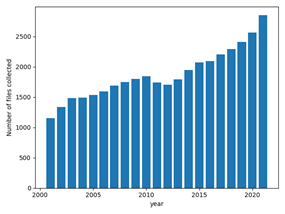
\includegraphics[width=\textwidth]{figures/byYear.png}
    \caption{Distribution of the number of files by year}
    \label{fig:byYear}

  \end{minipage}
  \hfill
  \begin{minipage}[b]{0.45\textwidth}
    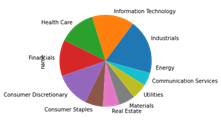
\includegraphics[width=\textwidth]{figures/byIndustry.png}
    \caption{Distribution of the number of companies by industry}
    \label{fig:byIndustry}

  \end{minipage}
\end{figure}


\begin{figure}[h!]
\centering
  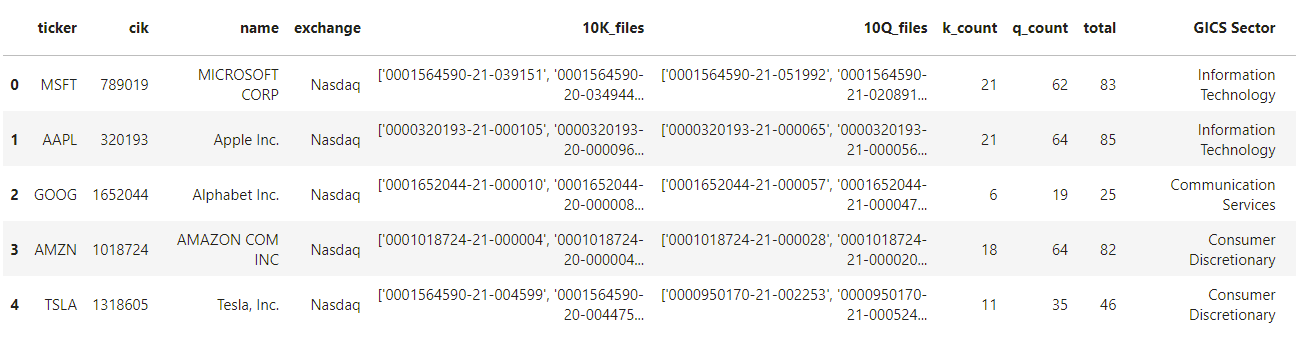
\includegraphics [width=\textwidth]{figures/meta.png}
  \caption{Snapshot of the Meta Information Sheet}
  \label{fig:meta}
\end{figure}



\subsection {Identity MD\&A Sections}

Due to the sheer size of the dataset and potentially formidable computational cost associated with the subsequent storage and search operations, it is necessary as a first step to filter the dataset in order to focus only on the most relevant information. In this case, we have already identified MD\&A section in these financial reports as the most relevant. Hence, the first step in our pipeline is to preprocess the raw data to extract the MD\&A section. 

To start, \emph{BeautifulSoup}\footnote{https://beautiful-soup-4.readthedocs.io} is employed to parse HTML files into raw texts. Then our system uses manually constructed rules to detect the start and end positions of the MD\&A section based on regular expressions. For 10-Qs, the MD\&A sections are typically found under the heading 'Part I.  Item 2' and for 10-Ks, the MD\&A sections are found under the heading 'Part II. Item 7'. After identification of the start and end position of a MD\&A section, the   

A total of 32,807 MD\&A sections (ca. 81\% of all files downloaded) are successfully extracted after the preprocessing step. There are 7,821 files that are disregarded by our system, because they do not contain a valid MD\&A section or our system could not identify either the start or the end position in the raw text file. Figure \ref{fig:MDAidentified} shows success rate of MD\&A extraction from raw files across all years. The earlier years have a much lower identification rates, as the early filings are not as standardized as compared to filings in recent years due to the tightening of the regulation requirements as already discussed in Section \ref{subsec:SEC}.

Figure \ref{fig:MDAlen} shows the distribution of length of the MD\&A sections by number of characters. The average length of MDA is ca. 70,217 characters. As an initial exploration, we extract the most frequent words by part-of-speech. Figure \ref{fig:NOUN} and Figure \ref{fig:VERB} in Appendix \ref{appendix:EDA} illustrate the top 100 nouns and verbs, respectively, from these MD\&A sections. The exploratory data analysis reveals some key characteristic of the MD\&A sections that the vocabulary is domain-specific and there seems to be certain patterns of language used in these texts.

\begin{figure}[!tbp]
  \centering
  \begin{minipage}[b]{0.45\textwidth}
    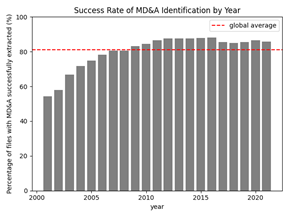
\includegraphics[width=\textwidth]{figures/MDAidentified.png}
    \caption{Success rate of MD\&A identification from raw files by by year}
    \label{fig:MDAidentified}

  \end{minipage}
  \hfill
  \begin{minipage}[b]{0.45\textwidth}
    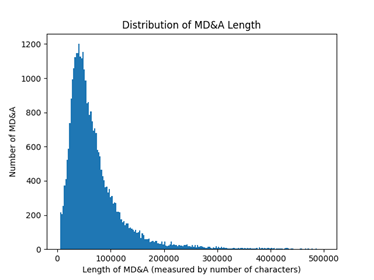
\includegraphics[width=\textwidth]{figures/MDAlen.png}
    \caption{Distribution of MD\&A lengths by number of characters}
    \label{fig:MDAlen}

  \end{minipage}
\end{figure}



\section{System Implementation} 
This section describes the implementation details of the pipeline. As illustrated in Figure \ref{fig:pipeline}, the input to the system consists of raw texts from the MD\&A sections. There are two main modules in the pipeline: Extraction and Clustering. The output of the system is the data model as described in Chapter 3. The pipeline is implemented in Python with external open-source libraries such as \emph{spaCy}\footnote{https://spacy.io/} for text processing and \emph{neo4j}\footnote{https://neo4j.com/product/neo4j-graph-database/} as the graph database for our data model. 

\begin{figure}[h!]
\centering
  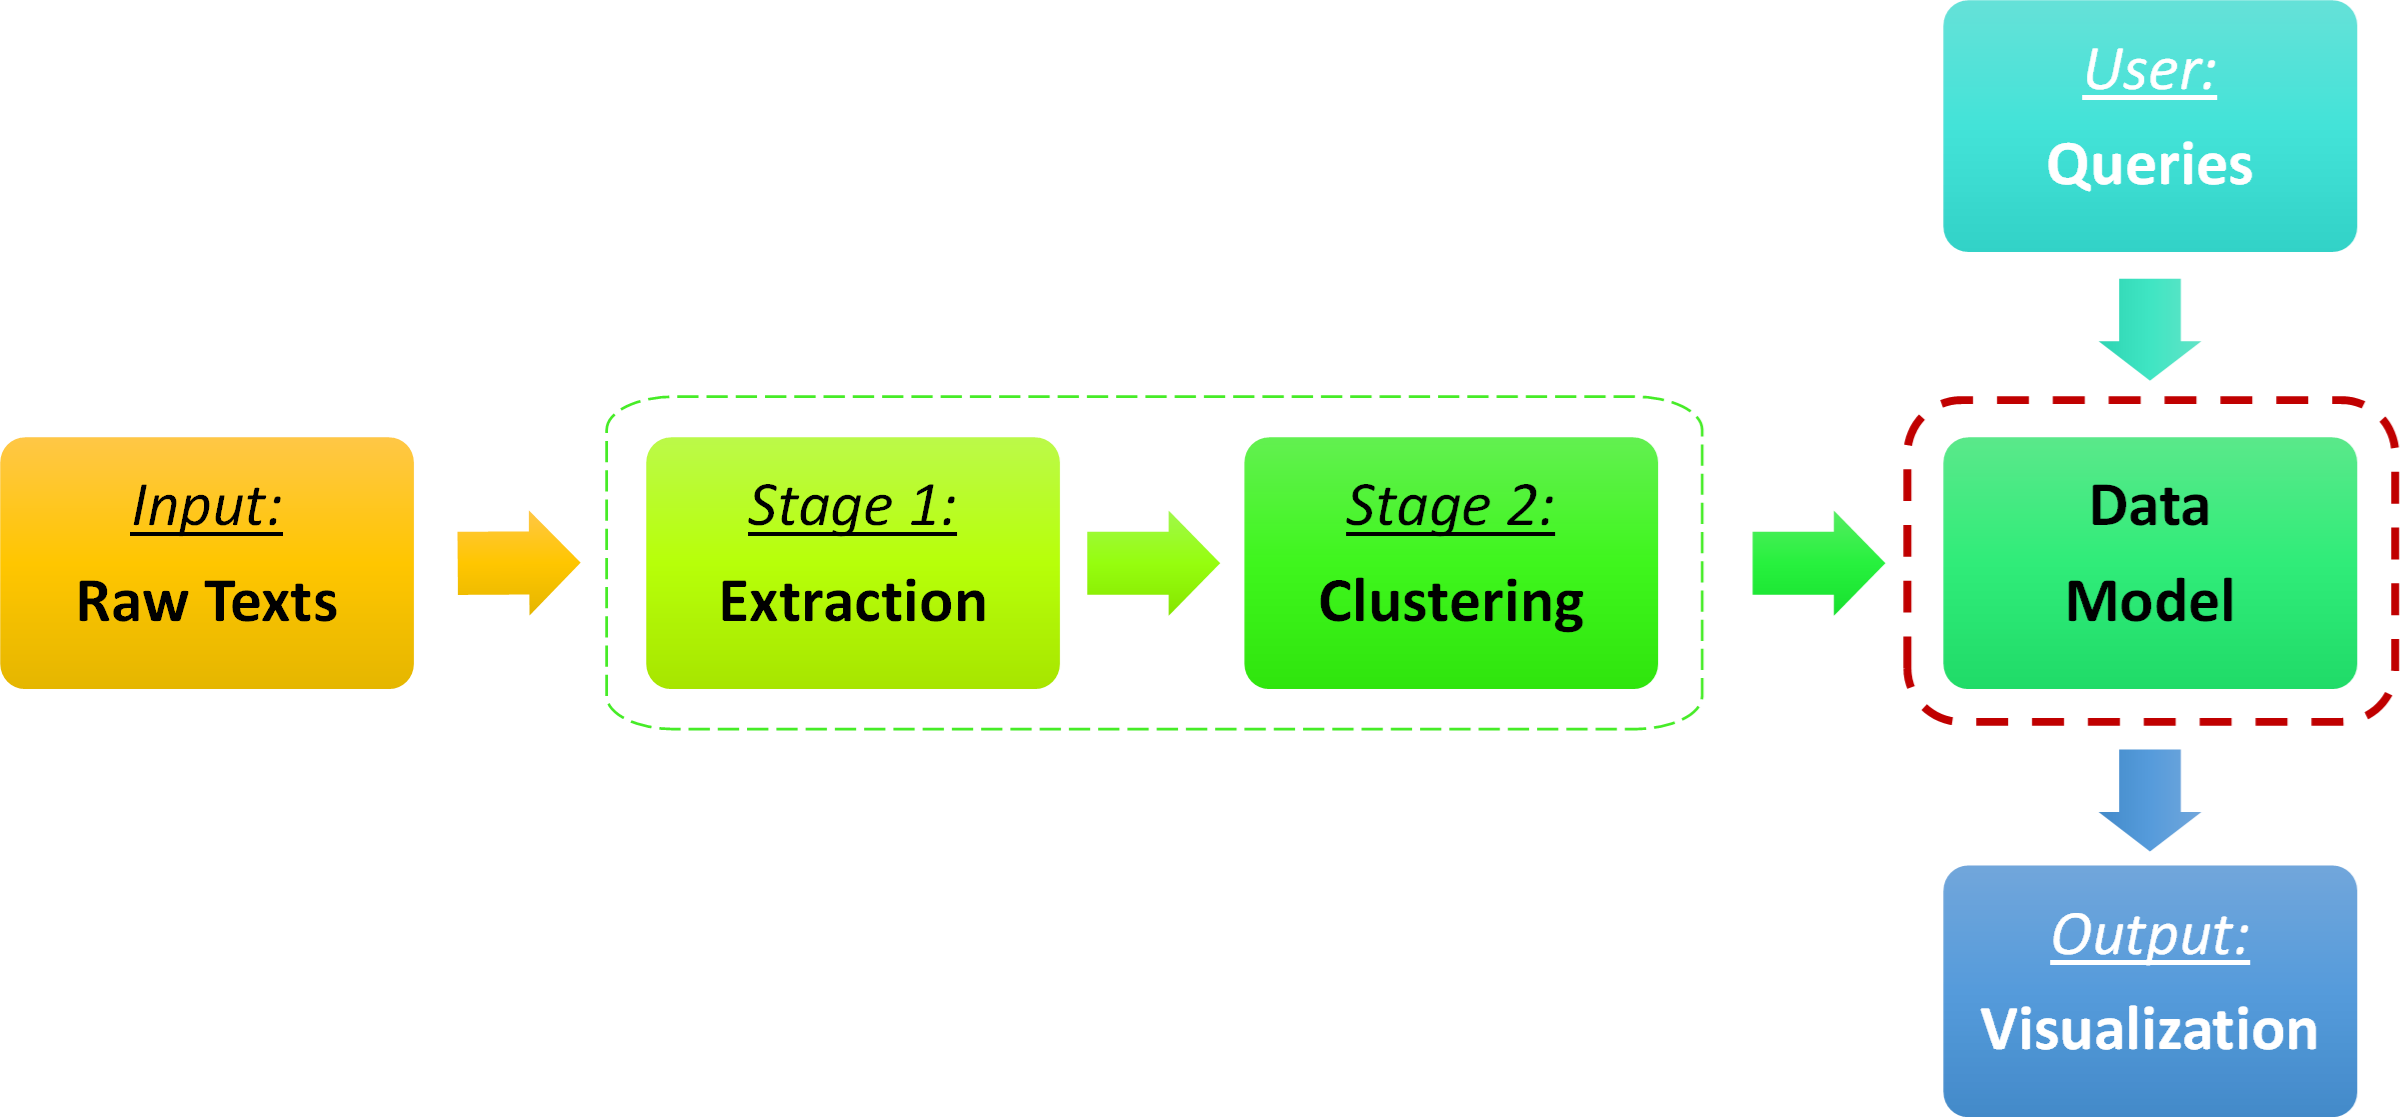
\includegraphics[scale=1.4]{figures/Pipeline_0.png}
  \caption{Illustration of Data Processing Pipeline}
  \label{fig:pipeline}
\end{figure}


\subsection{Extraction}
The extraction module identifies causal sentences and extracts causal factors in the form of noun phrases from these causal sentences. 

When a raw MD\&A text file is input into our pipeline, it is first split into sentences. Sentences that are too short (less than 50 characters), too long (more than 500 characters) or without any verb in the predicate, are discarded. The purpose of this preprocessing step is to filter off headings, section titles, bullet points, financial tables, and other text fragments, so that only proper, complete sentences are processed in this module.

As discussed in Section 3.3, only sentences containing causal explanations are regarded as relevant to our system's downstream processing. To extract these causal sentences, our system implements a linguistic pattern-based framework. The most commonly used causal markers from the MD\&A sections are manually identified. The current list includes the following causal connectives: 

\begin{itemize}
\item	verbs: \emph{result, affect, impact, cause, contribute, attribute, drive, relate, associate, reflect}
\item	non-verbs: \emph{due to, because, attributable to, as a result of, in connection with}
\end{itemize}

After the preprocessing step, each sentence is checked for the presence of causal connectives specified in the two lists above. For the sentences classified as causal, the system further process them to extract the cause and effect chunks. For example, in the sentence \emph{"For the quarter ended June 30, 2020, our advertising revenues declined due to the continued impacts of COVID-19 and the related reductions in global economic activity"}, the causal connective, \emph{"due to"}, qualifies the sentence as as a causal sentence. Accordingly, the template "\textbf{[effect chunk]} \emph{due to} \textbf{[cause chunk]}" is evoked. The sentence is parsed into the cause chunk, i.e., \emph{"the continued impacts of COVID-19 and the related reductions in global economic activity"} and the effective chunk, i.e., \emph{"For the quarter ended June 30, 2020, our advertising revenues"}, respectively. 

The system further extracts useful information from the cause and effect chunks. A topic of interest, e.g., \emph{"revenue"}, is identified from the effect chunk in the example sentence above. In addition,  noun phrases are extracted from the cause chunk with the help of SpaCy's default dependency parser, where noun phrases are defined as the \emph{"flat phrases that have a noun as their head"}\footnote{ https://spacy.io/usage/linguistic-features\#noun-chunks}. In laymen's term, it means that a noun plus the words describing the noun. In the example sentence quoted above, \emph{"The continued impacts", "the related reductions"} and \emph{"global economic activity"} are the noun phrases extracted from the cause chunk. 

Figure \ref{fig:chunks} provides a graphical illustration of the various parts of the example sentence identified by the extraction module. A total of 1,003,152 causal sentences are collected with a pre-defined list of topics, including the following terms: \emph{revenue, sale, cost, expense, margin, profit, earning, income,} and \emph{loss}. These causal sentences have an average length of 246 characters. From these causal sentence, a total of 5,069,900 noun phrases are extracted, of which 455,538 are unique. These unique noun phrases are to fed into the clustering module at the next stage of the pipeline for further processing.  

\begin{figure}[h!]
\centering
  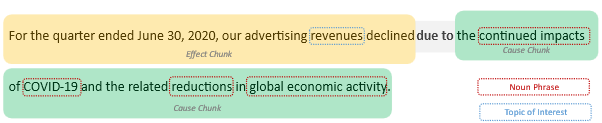
\includegraphics[width=\textwidth]{figures/CEchunks.png}
  \caption{Illustration of an example causal sentence and its cause and effect chunks with the identified topics of interest as well as noun phrases}
  \label{fig:chunks}
\end{figure}


The primary reasons for choosing a simple linguistic pattern-based system for causality extraction over the state-of-the-art deep neural models are three-fold. Firstly, training a deep neural model such as Bi-LSTM \cite{Li21BiLSTMCRF,Chen20} or BERT-CRF \cite {NTUNLPL20}, requires an annotated dataset of a reasonably large size, which we do not have. To commission such an annotation task based on our dataset is not only time-consuming but also costly. To leverage the existing datasets such as FinCaual \cite{FinCausal20} and SemEval \cite{SemEval07Task4, SemEval10Task8} is also not a viable option, because the tagging schemes are conceivably different from what this pipeline requires. 

Secondly, we recognize that interpretability and explainability are both very important for financial decision-making. Deep neural networks are black-box solutions inherently lacking interpretability. Their improved predictive accuracy has often been achieved through increased model complexity \cite{explainableAI2021}. In contrast, a rule-based system gives users the complete control over the causal sentence specification. It is not only transparent and accountable, but also computationally more efficient than deep neural models.  

Last but not least, we know from experience that the language style and sentence structures in these financial reports tend to conform to certain patterns, which can be exploited using rule-based heuristics. Our system may not generalize well in a domain agnostic scenario, however, it performs at a reasonable level of satisfaction for the domain-specific causal sentence extraction task at hand (see evaluation results in Section \ref{sec:evaluate}. In essence, our system is built based on the practicality of solving a problem using a minimal and frugal design.


\subsection{Clustering}
The clustering module of the pipeline processes the unique noun phrases collected from the preceding extraction module and group them into clusters according to their semantic similarity. These noun phrase clusters are referred to as concept clusters, as defined in Section 3.3.

For pretrained word embedding, our system uses the 'glove-wiki-gigaword-50' model \cite{glove2014}, downloaded from the Gensim-data repository\footnote{https://github.com/RaRe-Technologies/gensim-data}. The model has been trained on a combination of the Wikipedia 2014 dump and the Gigaword 5 corpus, with six billion uncased tokens, of which 400,000 are unique tokens\footnote{https://nlp.stanford.edu/projects/glove/}. Each word vector has 50 dimensions. To represent a noun phrase, our system takes the simple average of all word embeddings in the noun phrase and normalizes to a range of [-1,1] before feeding into the clustering algorithm.

For clustering, our system implements the SOM algorithm using the miniSOM library\footnote{ https://pypi.org/project/MiniSom/}. The number of neurons is decided based on the rule of the thumb \cite{SOM2019, SOM2014} that the total number of neurons should be $5\times \sqrt{N}$ where $N$ is the number of data points in the training set. In our case, $N = 455,539$, which is the number of unique noun phrases. Accordingly, a SOM with $3,364$ neurons arranged in a grid size of $58 \times 58$ is chosen. This particular topology is also chosen for the convenience of facilitating the final data visualization on a 2D map.

The network of the neurons are initialized with random weights and the neighborhood function is set to Gaussian. The optimal sigma and learning rate are determined through experimentation. The quantization error and topographic error (see Section 2.2.3) are used as the evaluation metrics for the SOM model performance. As illustrated in Figure \ref{fig:sig} and \ref{fig:lr}, we choose sigma = 2.5 and learning rate = 0.25 for our model. Furthermore, as illustrated in Figure \ref{fig:epoch}, we find that increasing the number of epochs (i.e. number of times that the SOM is trained on the entire dataset) does not affect the quantization error and the topographic error after the first pass. 

\begin{figure}
     \centering
     \begin{subfigure}[b]{0.3\textwidth}
         \centering
         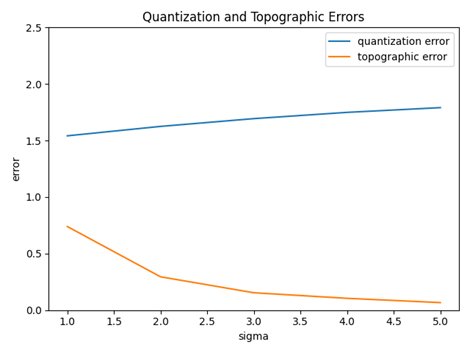
\includegraphics[width=\textwidth]{figures/SOM_sigmas.png}
         \caption{Sigma}
         \label{fig:sig}
     \end{subfigure}
     \hfill
     \begin{subfigure}[b]{0.3\textwidth}
         \centering
         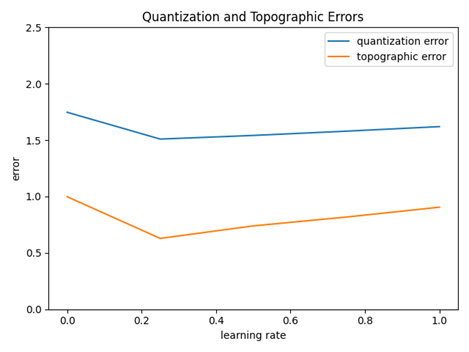
\includegraphics[width=\textwidth]{figures/SOM_learningrates.png}
         \caption{Learning Rate}
         \label{fig:lr}
     \end{subfigure}
     \hfill
     \begin{subfigure}[b]{0.3\textwidth}
         \centering
         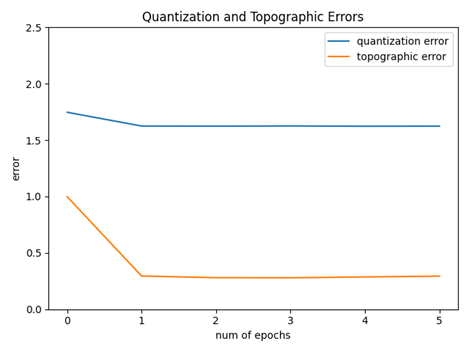
\includegraphics[width=\textwidth]{figures/SOM_epochs.png}
         \caption{Epoch}
         \label{fig:epoch}
     \end{subfigure}
        \caption{Quantization and Topographic Errors}
        \label{fig:experiments}
\end{figure}


Figure \ref{fig:distanceMap} shows the distance map of neuron weights of the SOM after training is complete. The color of each cell corresponds to the normalized sum of the Euclidean distances of that underlying neuron's weight to all its neighboring neurons'. It is effectively a visualization of how similar each neuron is to its neighbors and provides some indication for merging similar neurons into a larger clusters, i.e., the lighter regions on the map separated by darker boundaries.  

Figure \ref{fig:activationMap} shows the activation map of the SOM after training. The activation map is a matrix representation of the neurons network where the color intensity corresponds to the number of times that underlying neuron have been the winner during the competitive learning (see Chapter 2). In another words, the darker the cell is, the more data points has it seen during the training which have updated its weight. Therefore, it is also an indication of how many data points are associated with the underlying neuron.  


\begin{figure}
     \centering
     \begin{subfigure}[b]{0.45\textwidth}
         \centering
         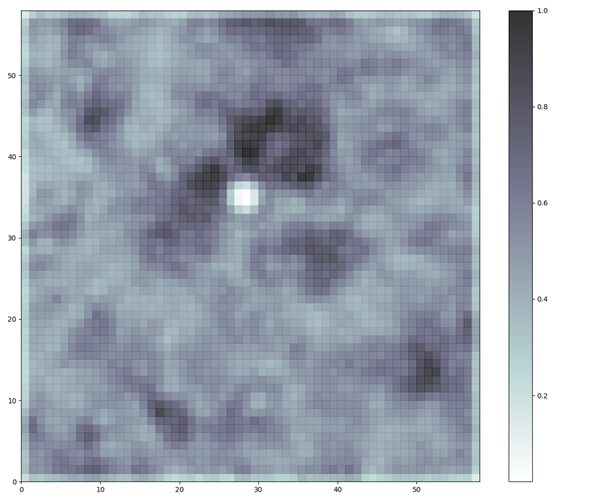
\includegraphics[width=\textwidth]{figures/SOM_distance.png}
         \caption{Distance Map}
         \label{fig:distanceMap}
     \end{subfigure}
     \hfill
     \begin{subfigure}[b]{0.45\textwidth}
         \centering
         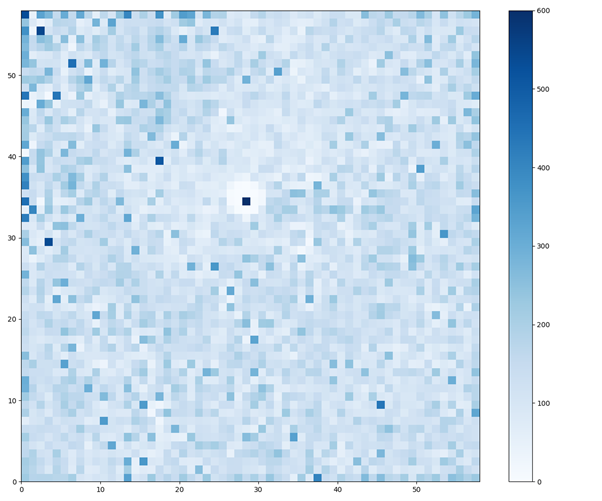
\includegraphics[width=\textwidth]{figures/SOM_activation.png}
         \caption{Activation Map}
         \label{fig:activationMap}
     \end{subfigure}
        \caption{2D map representations of the SOM after training. Distance Map is a visualization of how similar each neuron is to its neighbors. The Activation Map is a matrix representation of the neurons network where the color intensity corresponds to the number of times that underlying neuron have been the winner.}

\end{figure}

For the clustering module in our system, we choose SOM instead of K-means, as we do not know the optimal number of clusters, which is required as a hyper-parameters in the latter. In theory, we could use the Elbow's method \cite{elbow2020} to determine the optimal number of clusters, however, it does not provide a direct visual output illustrating the distances between the clusters. Some post-processing is needed in order to represent the clusters in a 2D map as the SOM output. 

Furthermore, due to the size of the dataset ($N=455,538$), hierarchical clustering is not suitable in terms of computation time and memory space required. The space complexity for hierarchical clustering is $O(N^2)$ with the storage of the similarity matrix in the RAM. In addition, the most naive implementation of the hierarchical clustering has a time complexity of $O(N^2 log N)$ \cite{clustering1999}. In contrast, both the SOM and the k-means algorithm have a linear time complexity of $O(NM)$, where M is the number of pre-specified clusters in K-means and the number of neurons in SOM, respectively. In terms of space complexity, K-means has $O(N+M)$ \cite{clustering1999} and SOM has $O(M^2)$ \cite{complexity2017}.  

[TODO: perform hierarchical clustering on the SOM output to reduce the number of clusters.] 

[TODO: to repeat the experiments with W2V 300 embeddings and check the quality of clustering]


\subsection{Data Model Implementation}

To implement the data model, we use Neo4j Community Edition 4.0.4 \footnote {https://neo4j.com/}, which is designed to handle graph data natively. We create different types of nodes and the corresponding edges according to the data model described in Chapter 3. 
More specifically, company nodes are created with the following properties: \emph{ticker, company name, sector classification}. Document nodes are created only for those that the MD\&A sections are identified. The document nodes have properties such as \emph{ticker, file name, file type (10-K or 10-Q)}. Edges are established between the company nodes and the document nodes where they share the same tickers. The edges are labeled with a property that specified the year of the document's publication.

For causal sentences identified by the causality extraction module of our system, causal sentence nodes are created with the following properties: \emph{raw text of the causal sentence, previous sentence, next sentence} (to provide some context). Edges are established between each causal sentence and the document it belongs to with a property that is labeled as \emph{topic}.

Noun phrase nodes are created for all the noun phrases extracted from the cause chunks of the causal sentences. Each node has the raw text of the noun phrase as a node property. Each noun phrase is linked with the causal sentence node where the noun phrase originates from. 

Finally, Concept cluster nodes are created based on the output from the clustering module of the system. Links are established between each concept cluster node and its constituent noun phrase nodes.
  
The resulting graph consists of $500$ company nodes, $32,807$ document nodes, $1,003,152$ causal sentence nodes, $455,538$ noun phrase nodes and $3,359$ concept cluster nodes. 



\section{Evaluation} \label{sec:evaluate}

\paragraph{Extraction Module:} To evaluate the performance of the causality extraction module, we take MD\&A sections from 3 documents and manually annotate the sentences which express causality. The performance statistics are shown in Table \ref{table:eval}.

The performance of the linguistic pattern based causality extraction module in our system is satisfactory with an overall precision of 90\%, recall of 89\% and F1-score of 90\%. Although it is slightly below the state-of-the-art deep neural models such as the Bi-LSTMs in \cite{Chen20} with a precision 92\% and recall 93\%, and the BERT-CRF model in \cite{NTUNLPL20} with F1 score of 95\%, our system is much simpler in design and requires much less processing. 


\begin{table} 
\small
\centering
\begin{tabular} {| m{2em} | m{5em} |m{5em} | m{3em} |m{3em} | m{3em} |m{3em} | m{3em} | m{3em} |}


\hline
 Doc & \#Casual Sentences Manually Identified & \#Causal Sentences Extracted by Model & \#TP & \#FP & \#FN & P\% & R\% & F1\%\\ 
\hline
\hline
1	& 98	& 94	& 88	& 6	& 10	& 94\%	 &90\%	 &92\% \\
\hline
2	&80    &	80	&74	&6	&6	&93\%	&93\%	&93\% \\
\hline
3	&74	&76	&63	&13	&11	&83\%	&85\%	&84\%\\
\hline
\textbf{All}	&\textbf{252}	&\textbf{250}	&\textbf{225}	&\textbf{25}	&\textbf{27}	&\textbf{90\%}	&\textbf{89\%}	&\textbf{90\%}\\
\hline
\hline
\end{tabular}
\caption{Performance statistics of the Extraction Module in our model, benchmarked against a small set of manually annotated sentences.}
\label{table:eval}
\end{table}



\paragraph{Clustering Module:} Since there is no ground truth for the clustering of noun phrases into concept clusters, we need to judge the quality of the concept clusters using common sense. We select 100 concept clusters at random and take 20 samples of noun phrases from each selected cluster. We inspect these clusters manually and conduct a sanity check to see if there is a semantic commonality among these in-cluster noun phrases. If more than half of these noun phrases in a cluster are semantically related to a common concept, then we mark this sample cluster as valid. Figure \ref{fig:cluster_samples} shows a few example clusters and the identified common concepts.

\begin{figure}[h!]
\centering
  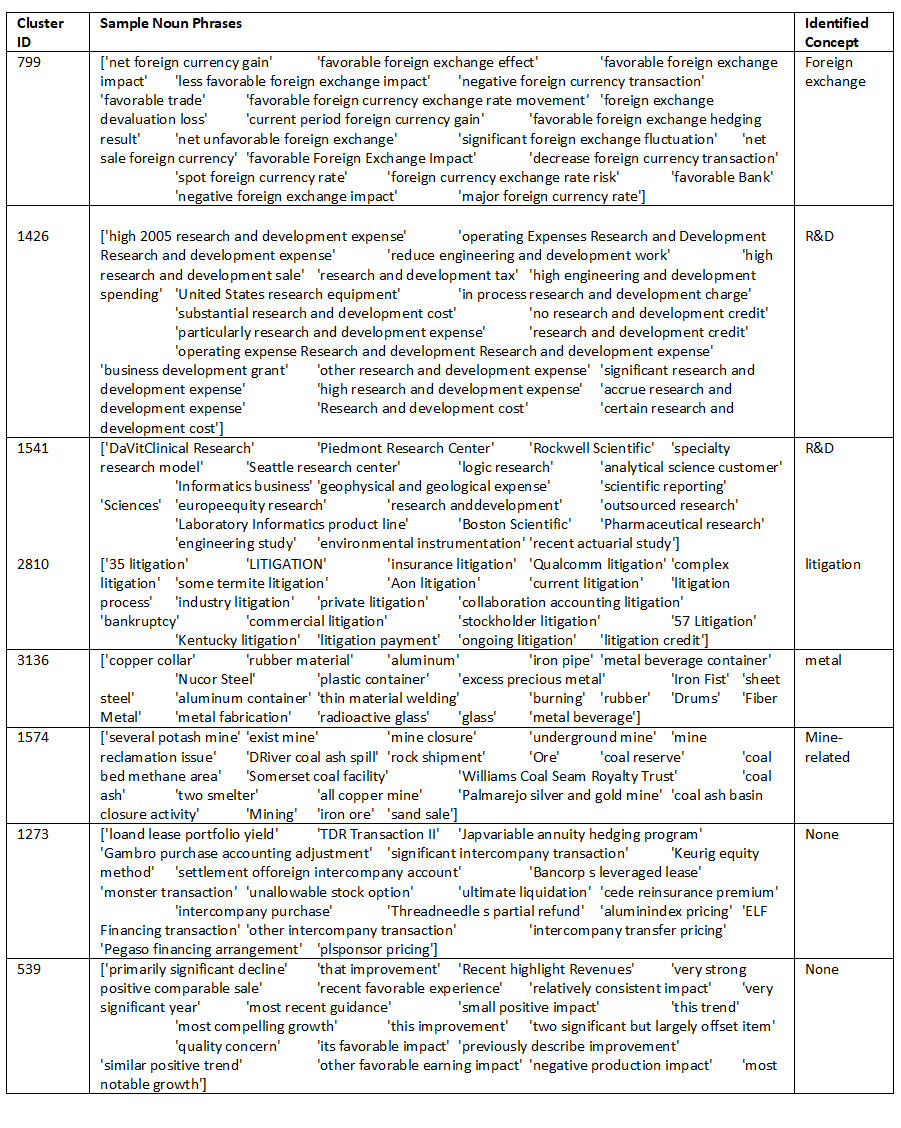
\includegraphics[width=\textwidth]{figures/cluster_samples.png}
  \caption{Examples of the concept clusters sampled from the clustering module output, with the manual identification of 'concepts' from the in-cluster noun phrase samples.}
  \label{fig:cluster_samples}
\end{figure}


This evaluation method is inherently subjective and is limited to the data points sampled from the training set. In the absence of objective ground truths, this evaluation method provides some preliminary indication of the clusters quality. Ultimately, the quality of the clusters is determined by the effectiveness and usefulness of the entire pipeline, which should be judged from the outputs of user queries. Section 4.4 demonstrates a few of such cases.



\section{Use Cases} 

This section demonstrates a few possible applications of the data model in helping to answer the specific investment research questions in Section 3.1. [Add more...]

\subsection{Company's Snapshot and Timeline Evolution}

We can represent the factors affecting a particular company's financial performance by the associated concept clusters distribution on the 2D map based on the SOM grid. When a company's ticker and a time period are specified, we create a query in the data model to collect all the relevant the noun phrases and their respective concept cluster indices, which are then mapped on the SOM grid as a visualization. For example, Figure \ref{fig:netflixlast4} illustrates four snapshots of Netflix in year 2018, 2019, 2020 and 2021, respectively. This way, we can trace the evolution of these factors over time. Moreover, we could also aggregate data at different granularity levels, as illustrated in Figure \ref{fig:netflix5yrs}, where each snapshot corresponds to a successive 5-year period. 

\begin{figure}
     \centering
     \begin{subfigure}[b]{0.45\textwidth}
         \centering
         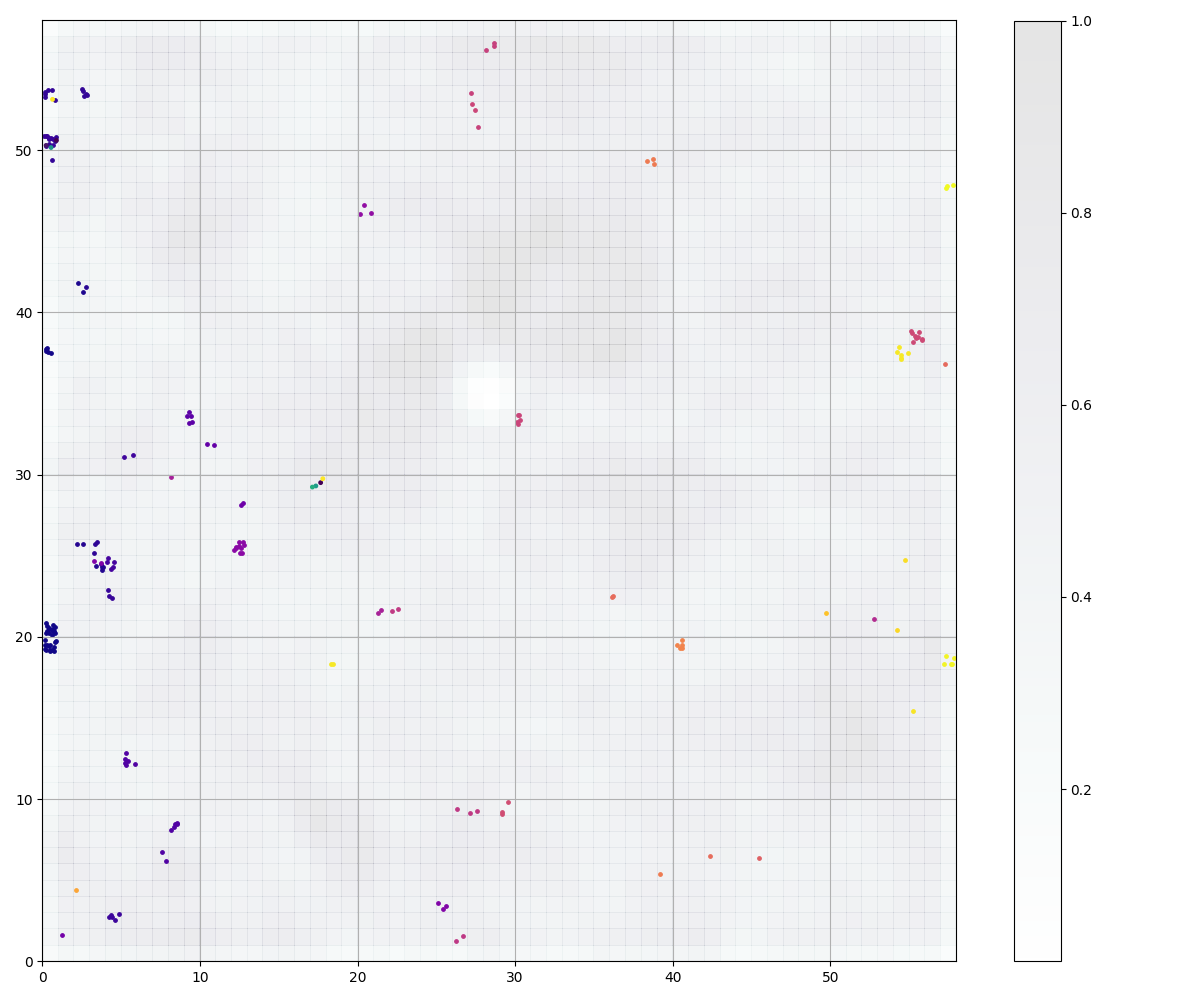
\includegraphics[width=\textwidth]{figures/NFLX_18.png}
         \caption{2018}
     \end{subfigure}
     \hfill
     \begin{subfigure}[b]{0.45\textwidth}
         \centering
         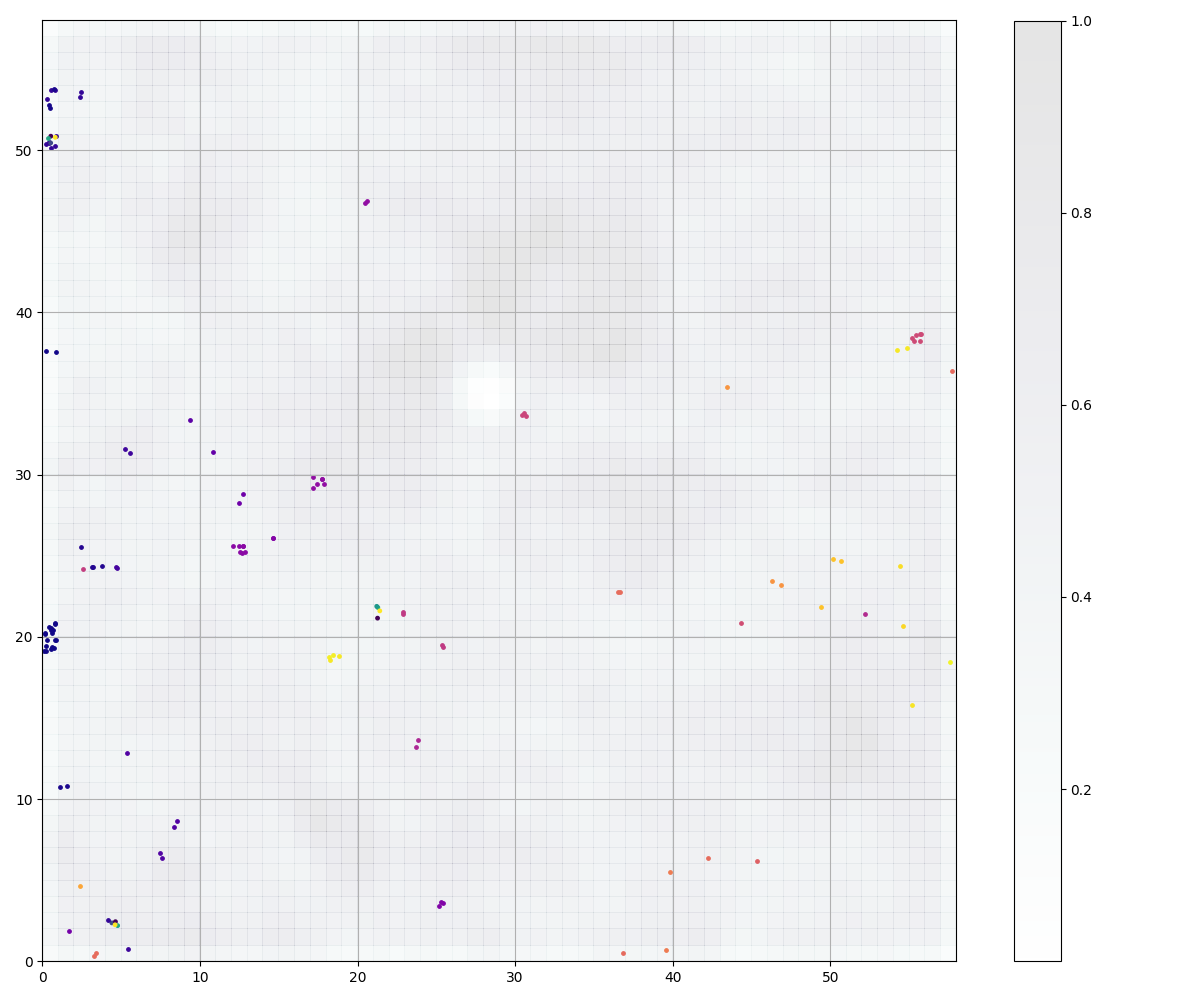
\includegraphics[width=\textwidth]{figures/NFLX_19.png}
         \caption{2019}
     \end{subfigure}
     \hfill
     \begin{subfigure}[b]{0.45\textwidth}
         \centering
         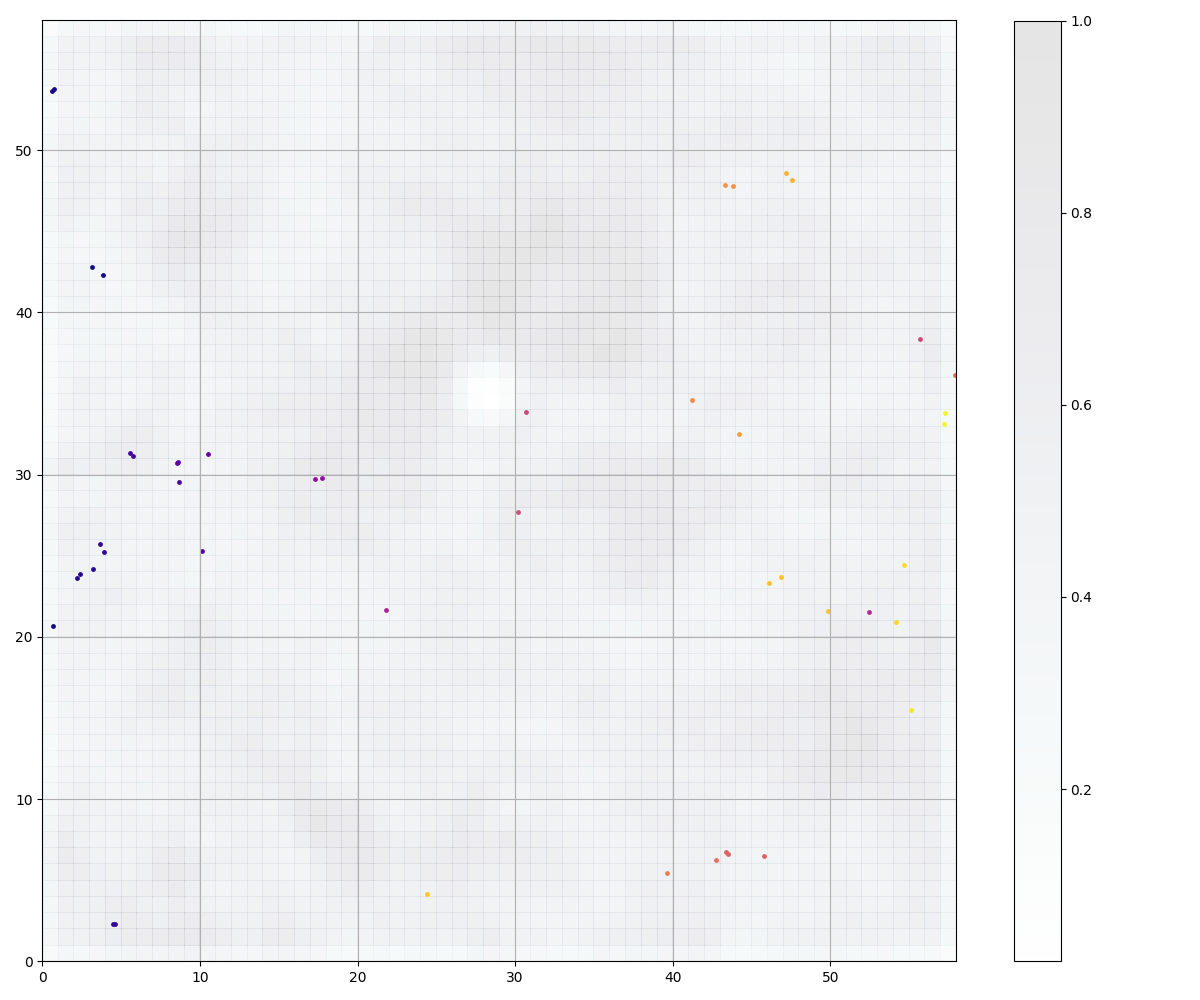
\includegraphics[width=\textwidth]{figures/NFLX_20.png}
         \caption{2020}
     \end{subfigure}
     \hfill
     \begin{subfigure}[b]{0.45\textwidth}
         \centering
         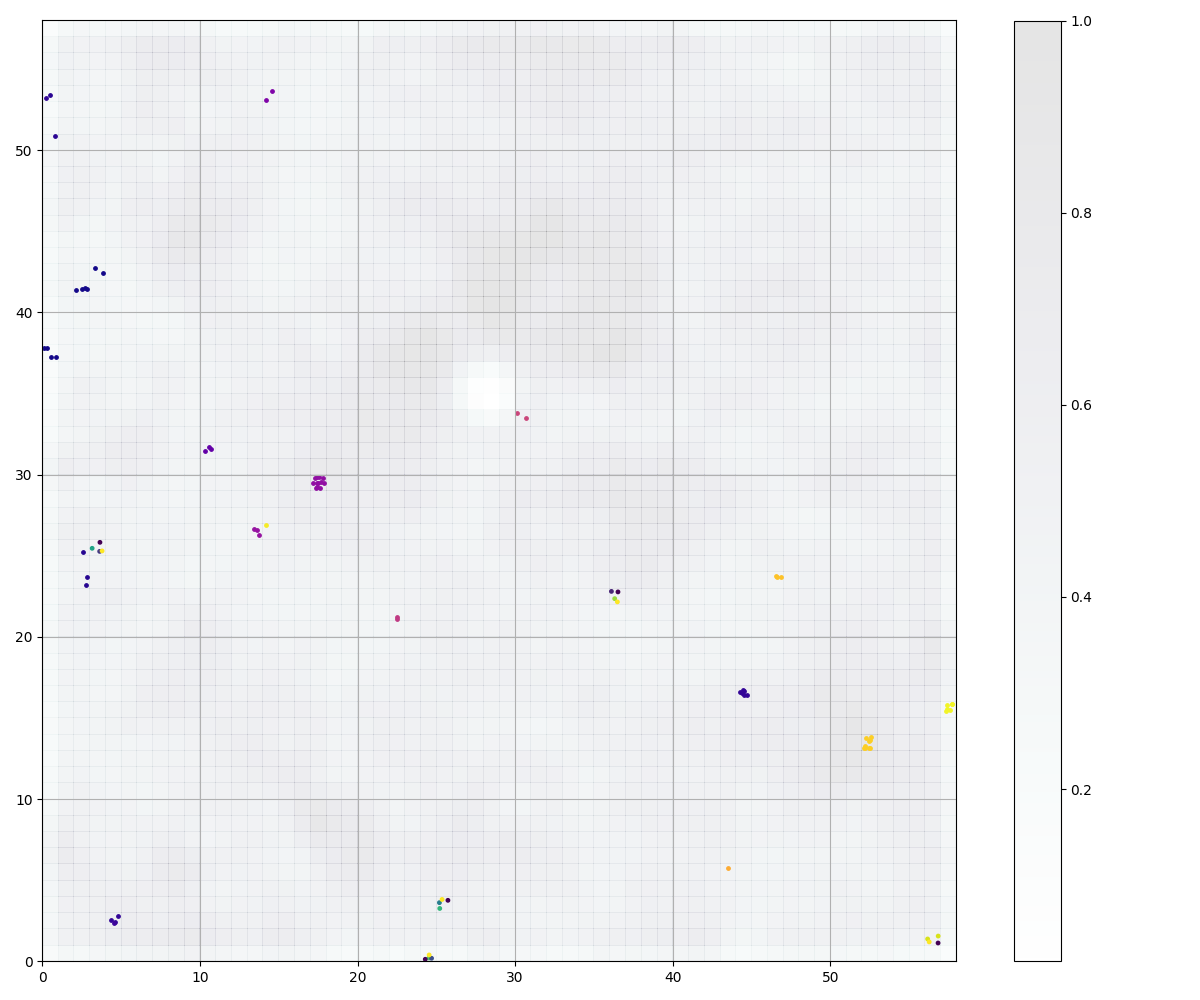
\includegraphics[width=\textwidth]{figures/NFLX_21.png}
         \caption{2021}
     \end{subfigure}
        \caption{Four annual snapshots of Netflix's causal factor map evolution from 2018 to 2021}
        \label{fig:netflixlast4}

\end{figure}




\begin{figure}
     \centering
     \begin{subfigure}[b]{0.45\textwidth}
         \centering
         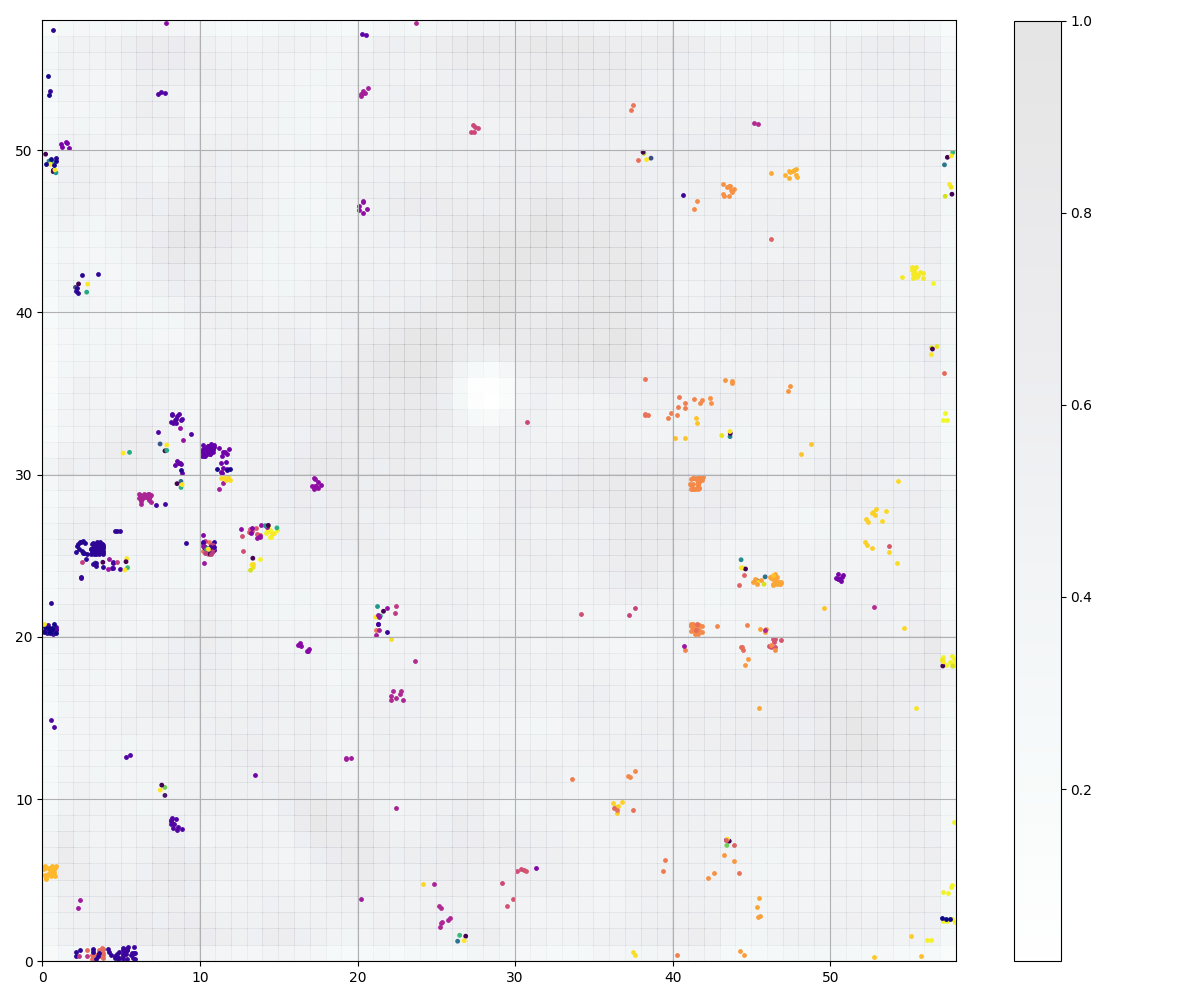
\includegraphics[width=\textwidth]{figures/NFLX_0205.png}
         \caption{2002-2005}
     \end{subfigure}
     \hfill
     \begin{subfigure}[b]{0.45\textwidth}
         \centering
         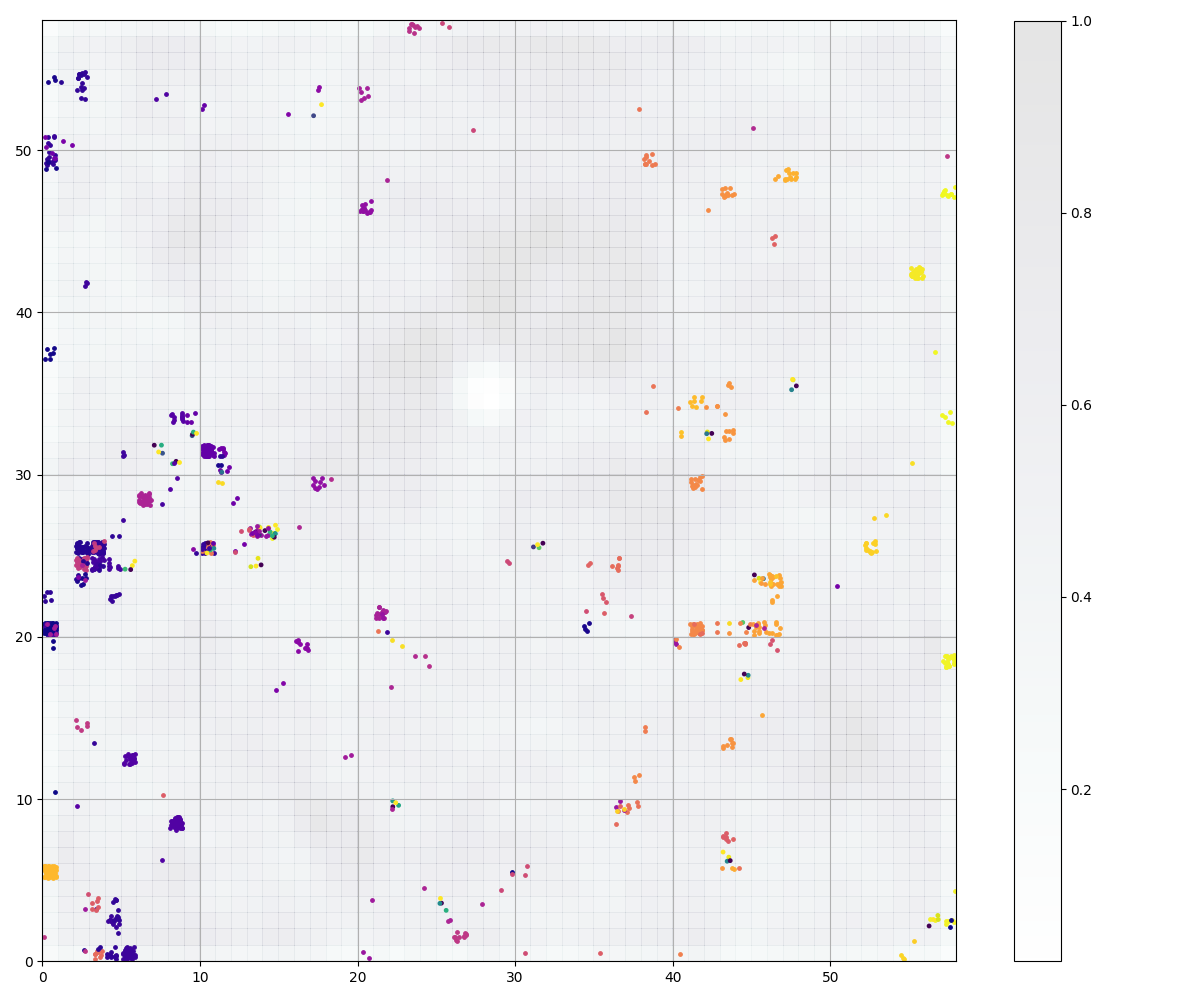
\includegraphics[width=\textwidth]{figures/NFLX_0510.png}
         \caption{2006-2010}
     \end{subfigure}
     \hfill
     \begin{subfigure}[b]{0.45\textwidth}
         \centering
         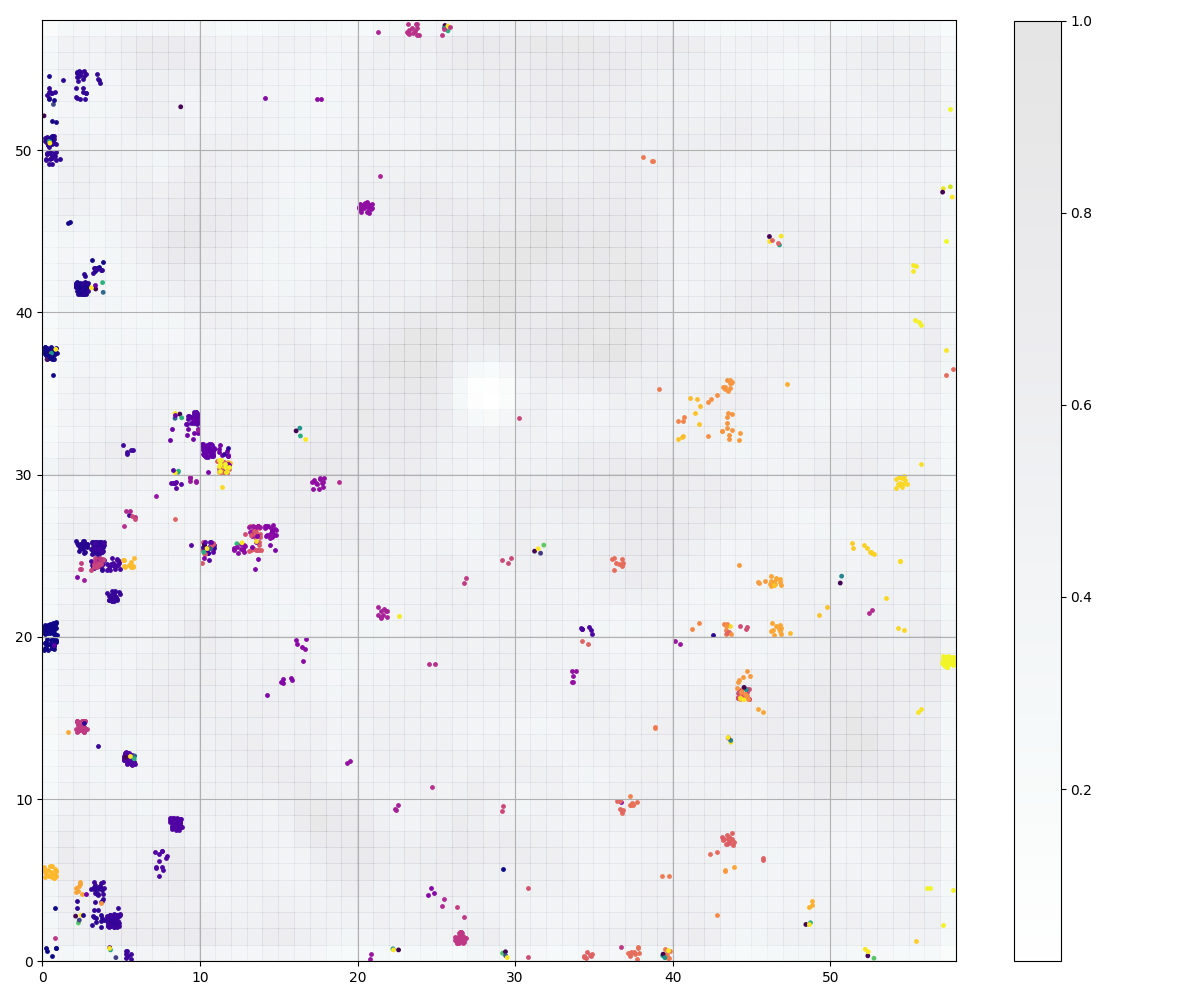
\includegraphics[width=\textwidth]{figures/NFLX_1015.png}
         \caption{2011-2015}
     \end{subfigure}
     \hfill
     \begin{subfigure}[b]{0.45\textwidth}
         \centering
         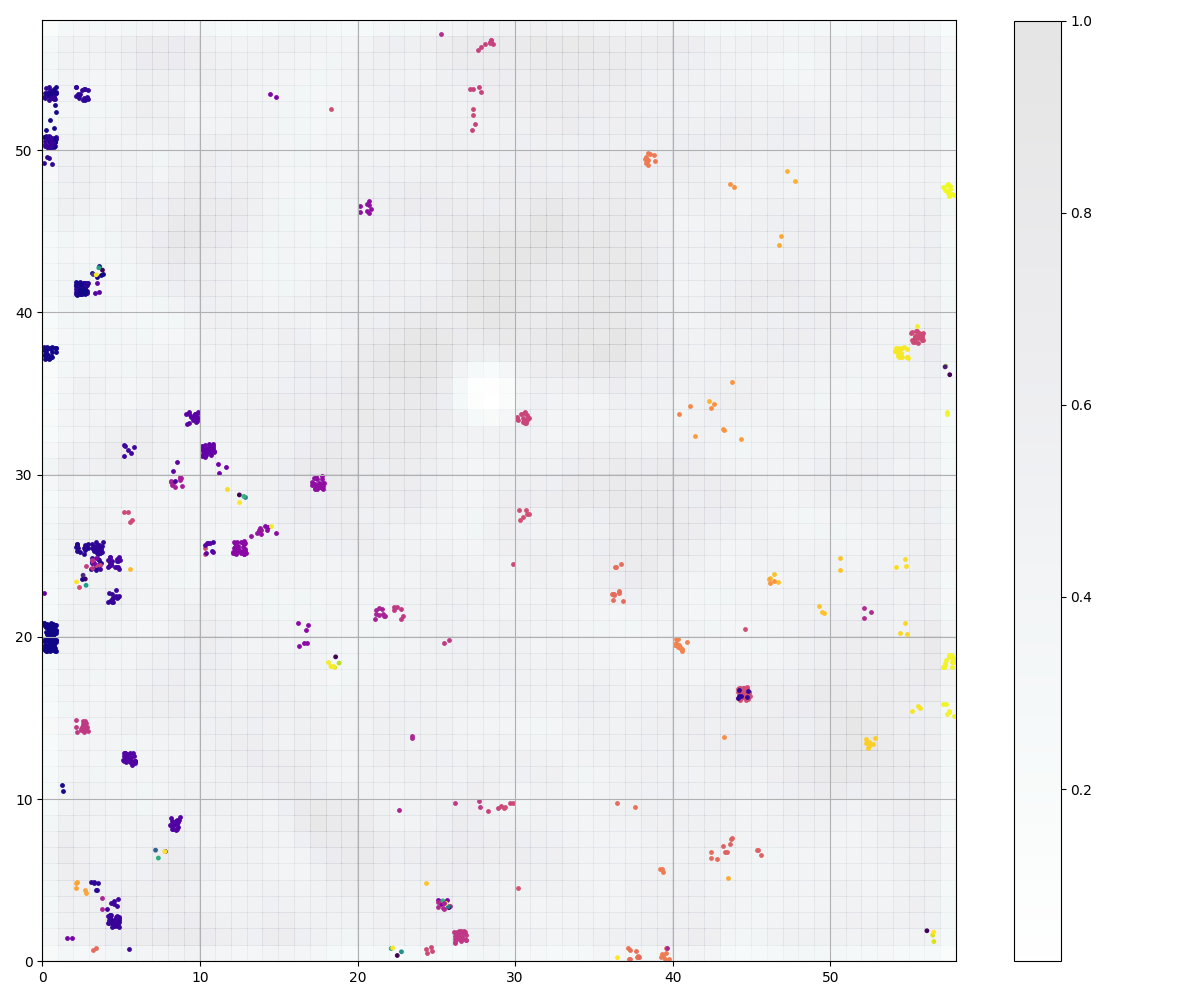
\includegraphics[width=\textwidth]{figures/NFLX_1521.png}
         \caption{2016-2021}
     \end{subfigure}

        \caption{Multi-year aggregated snapshots of Netflix's causal factor map in the last two decades.}
        \label{fig:netflix5yrs}

\end{figure}

By treating these snapshots as a company's signature, we can visually compare maps of two different companies and recognize their distinct patterns. Figure \ref{fig:nflx_ba} shows a side-by-side comparison of Netflix's and Boeing's signature maps aggregated over the last 20 years.  
[add comments on recognizable patterns]

\begin{figure}
     \centering
     \begin{subfigure}[b]{0.45\textwidth}
         \centering
         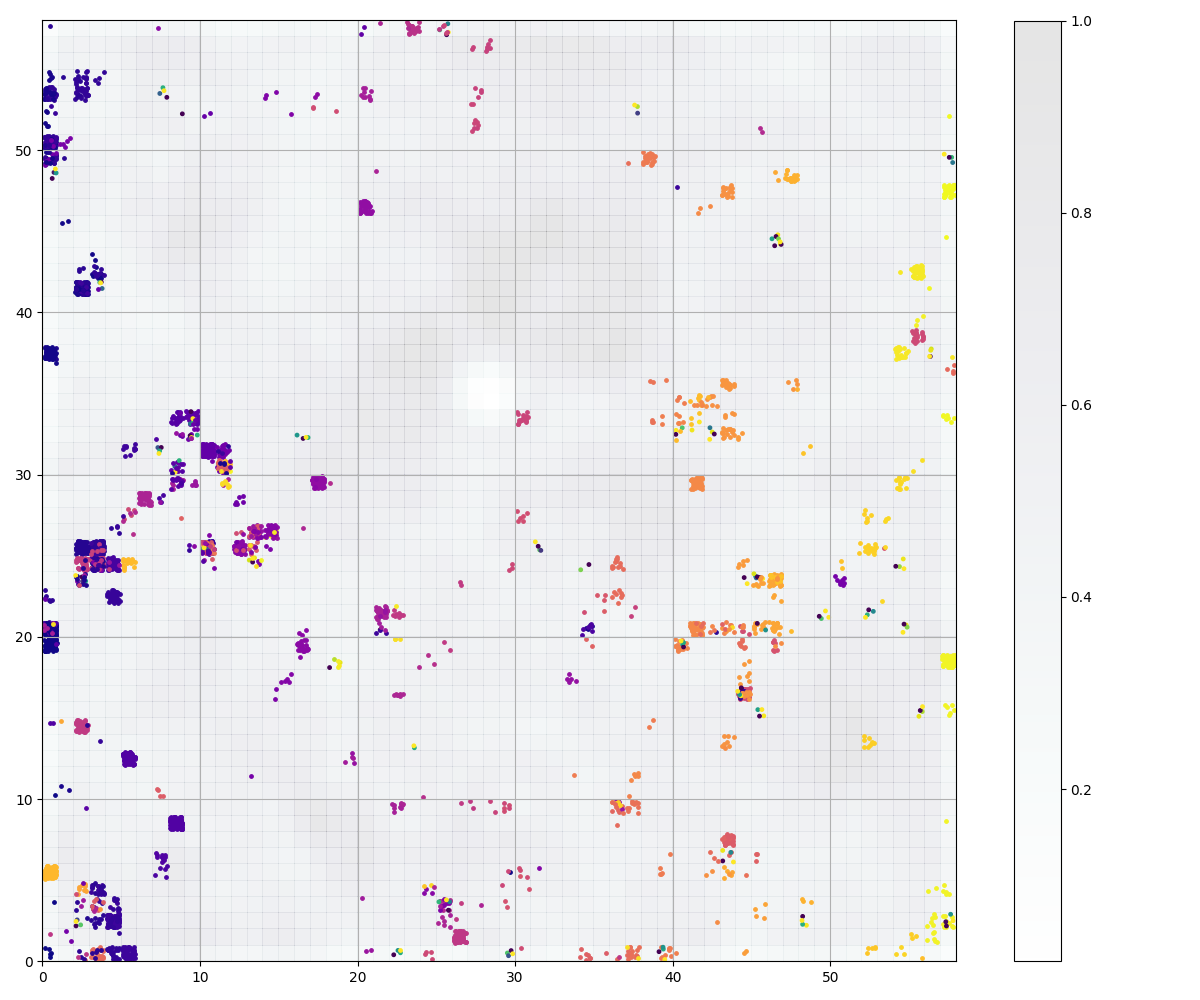
\includegraphics[width=\textwidth]{figures/NFLX_all.png}
         \caption{Netflix}
     \end{subfigure}
     \hfill
     \begin{subfigure}[b]{0.45\textwidth}
         \centering
         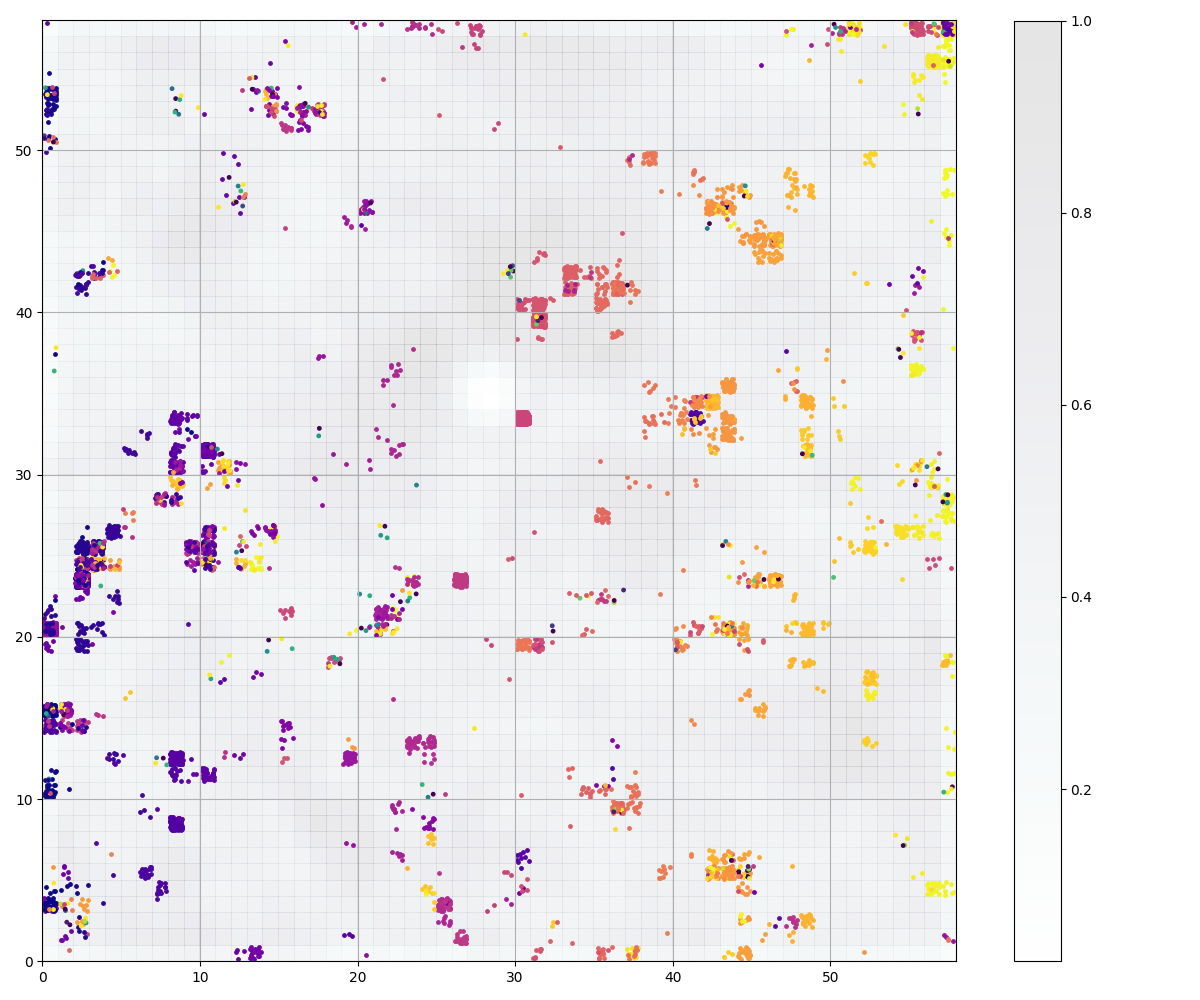
\includegraphics[width=\textwidth]{figures/BA_all.png}
         \caption{Boeing}
     \end{subfigure}

        \caption{Snapshots of Netflix vs. Boeing over the period 2001-2021}
        \label{fig:nflx_ba}
\end{figure}



\subsection{Comparable Companies}

Our data graph also enable users to find the most comparable peers for a target company. Each company can be represented by a vector where each dimension corresponding to a concept cluster. When the time period and topics of interest are specified, the number of links from a particular company to each concept cluster are counted. We calculate the cosine similarity between the target company and a set of potential candidates. These candidate companies can be ranked according to the similarity to the target company. As an illustration, Figure \ref{fig:simMatrix} shows the pairwise cosine similarity matrix of 50 companies. 

For the target company, JP Morgan Chase, for example, the top 5 most similar companies are:
\begin{itemize}
	\item 1. Wells Fargo \& Company (cosine similarity = 0.611)
	\item 2. At\&T (cosine similarity = 0.577)
	\item 3. Citigroup (cosine similarity = 0.531)
	\item 4. Chubb Ltd (cosine similarity = 0.501)
	\item 5. Marsh \& McLennan Companies (cosine similarity = 0.500)
\end{itemize}

[TO DO: discuss how it can be further improved by merging similar concept clusters together]

\begin{figure}
     \centering
     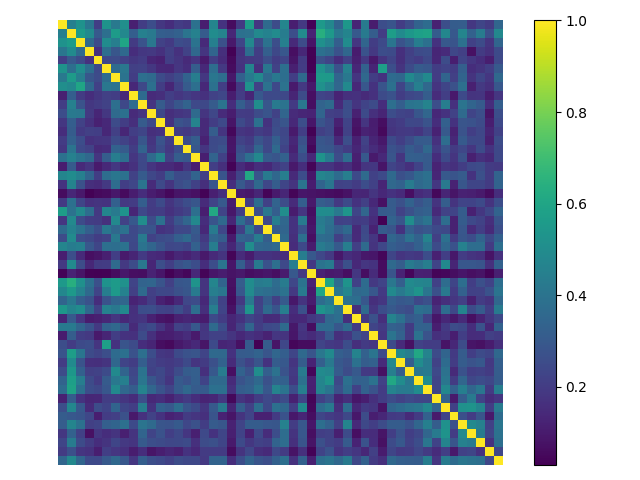
\includegraphics[width=0.7\textwidth]{figures/SimilarityMatrix.png}
     \caption{Cosine Similarity Matrix of 50 Companies}
	\label{fig:simMatrix}
\end{figure}




\subsection{Keyword Search for the Most Relevant Companies}
Another use case that can be envisaged is for the user to input a few key words and search for the most relevant companies. For instance, a user might be interested to find out which companies are most likely to be affected by price fluctuations in agriculture commodities with the specified input keywords: \emph{"wheat", "corn", "soybean"} and \emph{"meat"}. 

Our system first converts these keywords into word embeddings, which are fed into the clustering module one by one to find the most relevant set of concept clusters associated with these keywords. In the sample above, the set of concept clusters identified by our system are demonstrated in Table \ref{table:kwsearch}. Next, we define a query in Cypher to traverse the graph data model and collect all the companies that are connected to these identified concept clusters. We rank the companies by aggregating the total number of links to the set of concept clusters. 

\begin{table} 
\small
\centering
\begin{tabular} {| m{5em} | m{4em} |m{26em} |}
\hline
Keyword & \ Concept Cluster Index & \ Sample Noun Phrases from the Cluster\\ 
\hline
wheat & 2435 & \emph{rise dairy, acreage sale, Crop Protection, improved corn processing, seasonal purchasing, seasonal hog supply, weak harvest, cattle supply, lower plant acreage}\\ 
\hline
corn &2377 & \emph{new acreage, large harvest, concentrated phosphate crop, seasonal crop, grower activity, primarily cotton, less bountiful harvest, low hog harvest, Harvest} \\
\hline
soybean & 2435 & \emph{poor crop, potential sorghum duty deposit, oat supply, reduce crop production, increase cereal acre, reduce corn sale, wheat product, rise cattle, pork supply shortage}\\ 
\hline
meat & 2203 &\emph{pizza, Habit Burger Grill, deli item, taco, Premium Chicken Sandwiches, frozen pizza, meat ingredient, Chicken, Chipotle restaurant} \\ 
\hline
\end{tabular}
\caption{Concept Clusters identified by the clustering}
\label{table:kwsearch}
\end{table}


In the above example, our system outputs the following companies as the most relevant to the input search terms:

\begin{itemize}
	\item 1. General Mills: manufacturer and marketer of branded consumer foods (234 links)
	\item 2. Tyson Foods: meat processor and marketer (203 links)
	\item 3. Campbell Soup: processed food and snack company (151 links)
	\item 4. Zoetis: a global animal health company (109 links)
	\item 5. Archer-Daniels-Midland: food processing and commodities trading corporation (104 links)
\end{itemize}


Table \ref{table:searchexamples} shows a few other examples in keyword search. Note that the output of this search is only meant for providing a rough indication ... [add comments]

\begin{table} 
\small
\centering
\begin{tabular} {| m{15em} |m{25em} |}
\hline
Keywords & \ Top 5 Most Relevant Companies \\ 
\hline

aircrafts, flights, fuel price & Alaska Air Group, Southern, American Airlines Group,  
United Parcel Service, Southwest Airlines \\
\hline
cloud computing, business analytics, cloud storage, data management &
Amazon, Akamai Technologies, CF Industries Holdings, Northrop Grumman, Equinix \\
\hline
global supply chain disruption, inflation, pandemic, Covid-19 & Prudential Financial, Metlife, Sysco, United Parcel Service, Cognizant Technology Solutions\\
\hline
\end{tabular}
\caption{Further examples in keyword search}
\label{table:searchexamples}
\end{table}





